%!TEX root = ../report.tex

\chapter{State of the Art}

\section{Existing sonar image matching techniques}
\begin{itemize}
 \item 
\end{itemize}


\section{Deep neural network}
From wikipedia \cite{wikidnn} deep neural networks (DNN) are type of artificial neural networks which can have many layers between their input and output. The DNN can be used to estimate the underlying mathematical manipulation
which maps the output to the input in, a manner which is more of less consistent across all the samples. The network calculate for all the layers the probability of each outputs and then the correct label can be displayed as output 
if the probability is above a certain threshold. Each mathematical manipulation can be considered a layer, a DNN can have many such operating layers, that is why it is named deep neural network. For example, in our scenario two sonar 
image patches are given as input to the DNN, it will calculate different features from both image patches and at the end it will decide if the derived features are similar then the input patches are similar.

\section{Convolutional network}
\cite{wikicnn} 
Describe the parts of the conv net and the roles of the layers. Such as fully connected layers, max pooling, average pooling, activation functions such as Relu and Sigmoid. Initializers ?

Inspired by  \cite{stateoftheart} following notation for CNN layers are used to describe components of the architectures: Conv(Nf,Fw xFh) is a convolutional layers with Nf filters of width Fw and height Fh.
A max-pooling layer is represented by MP(Pw, Ph) where PwxPh is the sub-sampling size of the layer, and FC(n) is a fully connected layers where n represents output size.

\section{Siamese network}
In 1993 the concept of a new artificial neural network called Siamese network was introduced by Bromley et al. \cite{bromley1994signature}. Siamese network consists two identical sub-networks which are joined at the output.
During training stage one input each is connected to each of the subnetworks. The main idea here is that the subnetworks (also called branches) are trained simultaneously and extract features from the inputs.
While the shared neurons are capable of measuring the distance between the two extracted feature vectors by each branches. If the predicted distance between two feature vectors is lesser than a threshold then it can be considered 
that the inputs are similar. Authors used this concept to compare two signatures in \cite{bromley1994signature}. One of the signature was previously obtained from the authentic owner (up to 6 signatures were recorded). This was then used to compare with a new signature
to verify if the both persons are same or not, as precaution against forgery. Authors implemented the Siamese network to be able to extract and compare different features of the two signatures and if the output is within a threshold then
they were considered matching. If not then it was most likely a forgery.

\section{CNN for learning similarity function}

Zagoruyko et al. have demonstrated that CNNs can be directly deployed to learn the underlying similarity function to be able to determine that two input images/patches are different instances of same object or not, 
without any help from hand designed features. The scarcity of accurate hand designed features for sonar images motivated Valdenegro et al. to evaluate similar approach as Zagoruyko et al. and encode a CNN for sonar image comparison.

Valdenegro et al. \cite{stateoftheart} evaluated two architectures, a two-channel network and a Siamese network. The architectures \ref{fig:two_channel_only_siamese} were based on the work from zagoruyko et al. \cite{zagoruyko2015learning}.
A grid search was used over pre-defined set of parameters which define the network structure. The final two channel network structure presented in the paper for predicting binary classification score was as follows,
Conv(16, 5 x 5)-MP(2, 2)-Conv(32, 5 x 5)-MP(2, 2)-Conv(32, 5 x 5)-MP(2, 2)- Conv(16, 5 x 5)-MP(2, 2)-FC(64)-FC(32)-FC(1). Similarly grid search was also conducted for Siamese network structure for classification score. The structure for each 
of the branches or sub-network is as follows, Conv(16, 5 x 5)-MP(2, 2)-Conv(32, 5 x 5)- MP(2, 2)-Conv(64, 5 x 5)-MP(2, 2)-Conv(32, 5 x 5)-MP(2, 2)-FC(96)-FC(96). The output features from the branches were then concatenated to form 192 
element vector. This was then passed through a decision network with FC(64)-FC(1). For both two channel and Siamese network the final FC(1) layer had Sigmoid \cite{kerassigmoid} activation function and binary cross entropy loss\cite{kerascrossentropy}
function. 

Not very complex network structures were used. In general sense, adding more layers in the network does add more non-linearity to it and in some cases, that improves the performance of the network. So in theory, more advanced networks or loss 
functions which help extracting more discriminative and patch invariant features, should improve the results even further.

\begin{figure}[ht]
\centering
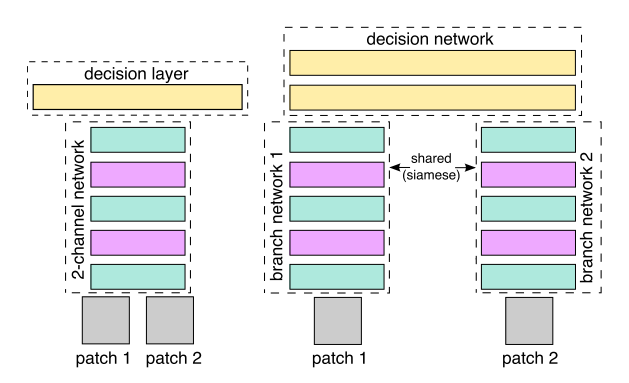
\includegraphics[height=6cm]{images/densenet/two_channel_only_siamese.png}
\caption{Two channel(left) and Siamese CNN architectures used in Valdenegro et al., though the figure and inspiration is from \cite{zagoruyko2015learning}}
\label{fig:two_channel_only_siamese}
\end{figure}
